% !TeX root = ../technical_paper.tex


\section{方案论证与设计}

\subsection{总体方案}

本作品采用 GD32G553 主控、GD32C113 BMS 和 GD32VW553 无线模块构成的三节点协同架构。GD32G553 负责系统调度、BMS 数据接收与转发、PWM 输出及采样管理；GD32C113 负责电池测量、保护判断、均衡控制和 SOC 估算；GD32VW553 负责无线通信和远程监控。三者通过 CAN FD 与 UART 连接，构成从电池状态采集到远程监控展示的闭环。

该方案将实时性要求高的控制与保护任务（主控、BMS）和低实时性的交互任务（无线）分离，避免单 MCU 软件耦合过深，降低调试和扩展难度。

\begin{figure}[htbp]
  \centering
  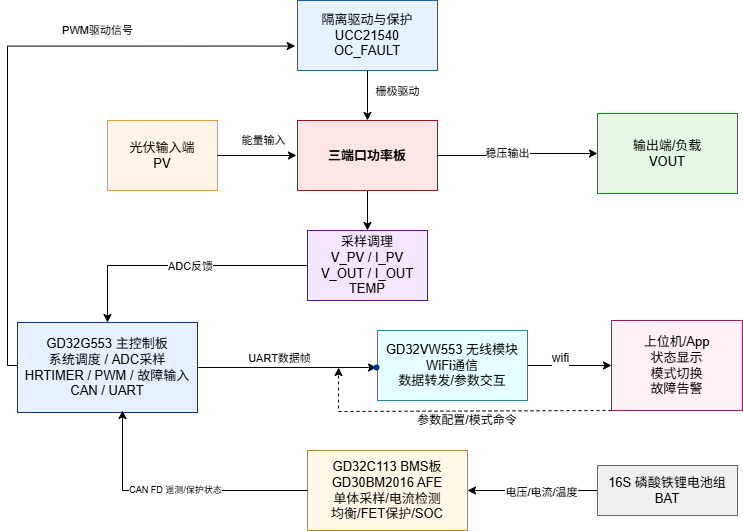
\includegraphics[width=0.95\textwidth]{images/流程图架构图/系统总体架构示意图.drawio.png}
  \caption{系统总体架构示意图}
  \label{fig:system_architecture}
  \vspace{0.2em}
  {\small 资料来源：作者绘制。}
\end{figure}

% TODO: 插入系统数据流关系图
\begin{figure}[htbp]
  \centering
  \centerline{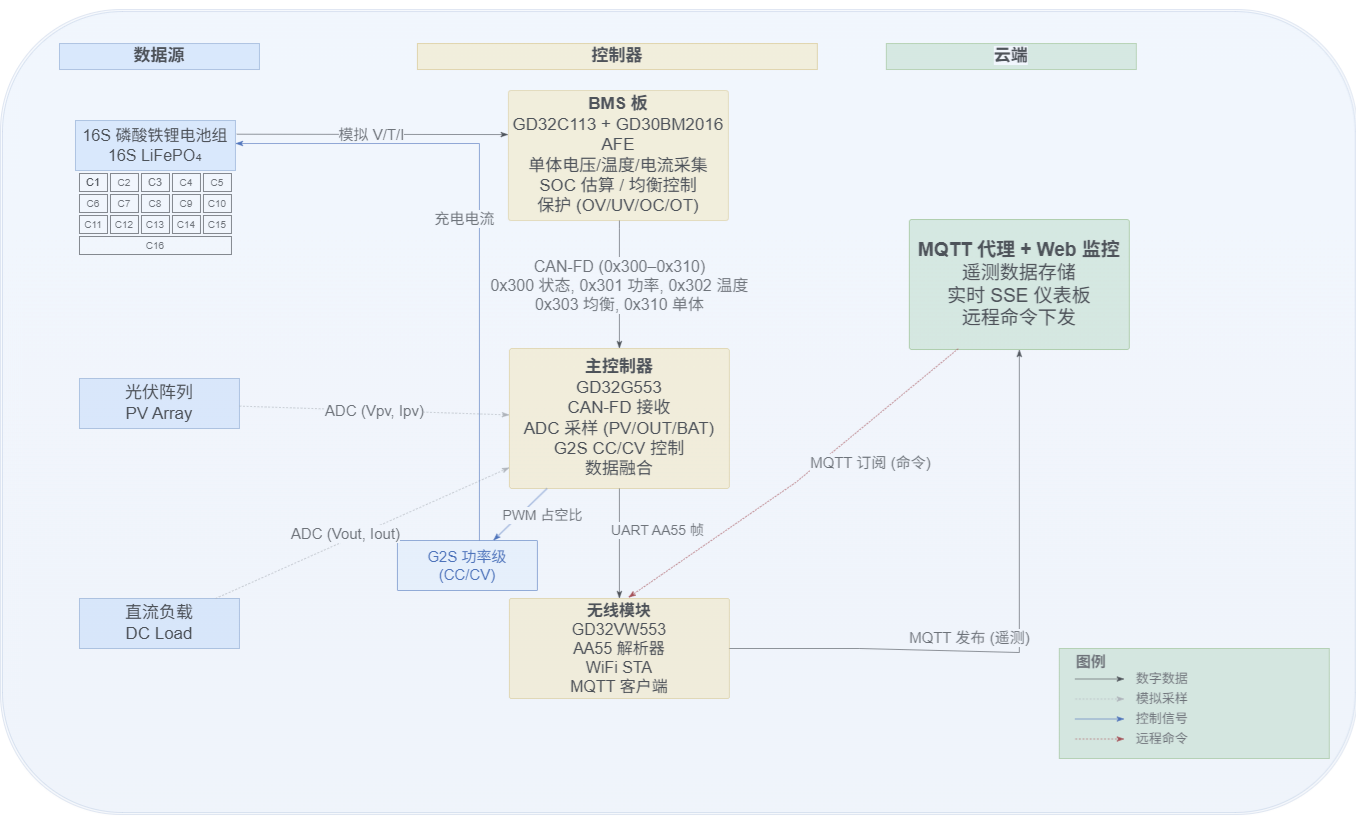
\includegraphics[width=0.88\textwidth]{images/流程图架构图/BMS端到端数据流.drawio.png}}
  \caption{系统数据流关系}
  \label{fig:data_flow}
  \vspace{0.2em}
  {\small 资料来源：作者绘制。}
\end{figure}

系统的核心设计思想是将强实时任务与弱实时任务分离。功率变换闭环、PWM 更新和快速保护由 GD32G553 就近完成；电池状态估算、均衡和电池侧保护由 GD32C113 独立完成；无线通信、数据记录和人机交互由 GD32VW553 承担。通过任务分层，系统避免了无线通信和日志处理对功率控制中断的干扰。


\subsection{主要参数与系统规格}

表 \ref{tab:spec} 给出了本系统的目标规格。

\begin{table}[htbp]
  \centering
  \caption{系统目标规格}
  \label{tab:spec}
  \begin{tabular}{@{}llp{7.2cm}@{}}
    \toprule
    \textbf{项目} & \textbf{设计目标} & \textbf{说明} \\
    \midrule
    光伏输入电压   & 约 36~V 等级            & 面向低压光伏输入场景，便于与实验电源和光伏模拟源联调 \\
    储能电池电压   & 约 48~V 等级            & 单体标称电压 3.2~V，满充电压约 58.4~V，放电截止附近约 40~V \\
    直流母线电压   & 约 200~V 等级（规划）    & 为后级交流逆变预留直流母线电压裕量，当前阶段尚未实现 \\
    交流输出       & 220~V/50~Hz（规划目标）  & 后级逆变单元为远期规划，当前仅预留控制接口与硬件位置 \\
    额定功率       & 约 200~W（前级规划）    & 依据前级功率器件、电感和散热能力预估，待闭环验证 \\
    控制平台       & GD32G553/GD32C113/GD32VW553 & 主功率控制、BMS、无线监控分工 \\
    保护功能       & 过压/欠压/过流/过温/通信异常 & 硬件保护与软件状态机结合 \\
    \bottomrule
  \end{tabular}
\end{table}

\subsection{方案选择与论证}

本作品采用多 MCU 协同方案，主要基于以下考虑。

\begin{enumerate}[label=\arabic*、, leftmargin=*, itemsep=0.8ex, parsep=0pt, topsep=0.5ex]
  \item \textbf{实时控制与远程交互的实时性要求不同。}
  主控和 BMS 的采样、判断、保护动作需要较高实时性，而网页展示、参数配置和日志传输允许较低刷新频率。若将两类任务集中在单一控制器内，容易造成中断拥塞、控制周期抖动和异常响应延迟。

  \item \textbf{电池安全控制需要独立闭环。}
  BMS 不应仅作为主控的一个附属采样模块，而应独立完成测量、保护、均衡和 FET 策略。这样在发生过压、欠压、过温、采样异常或通信异常时，BMS 可立即执行降级和关断策略，保证电池安全优先。

  \item \textbf{监控系统不应干扰底层控制。}
  无线通信、数据展示和参数配置本质上属于非实时任务，如果和底层保护逻辑耦合过紧，一旦网络阻塞或页面刷新异常，就可能影响核心控制链路。因此，需要把监控链路从控制链路中剥离出来。

  \item \textbf{模块化设计有利于后续扩展。}
  采用主控、BMS、无线模块分层设计后，后续若要增加新的采样项、告警类型或页面字段，只需扩展对应模块即可，不必重构整个系统。
\end{enumerate}
因此，本作品最终选择"主控负责调度与转发、BMS 负责安全与状态、无线模块负责展示与交互"的系统分工方式，并通过统一数据格式与状态编码将各模块连接起来。
\subsection{控制芯片分工}

\subsubsection{GD32G553 与主功率控制}

GD32G553 主控工程采用四层解耦架构，将系统划分为 APP 层、Middleware 层、Protocol 层和 HAL 层。该结构的核心思想是让应用逻辑、数据管理、协议处理和底层驱动相互隔离，从而提升代码清晰度和可移植性。

在 APP 层，系统通过统一调度器组织各模块运行，包括 BMS 数据转发、心跳帧输出和 HRTIMER PWM 任务等；在 Middleware 层，采用发布/订阅式数据总线组织系统内部数据流，使数据生产者与消费者解耦；在 Protocol 层，完成 CAN FD 帧解析与 UART AA55 帧封装；在 HAL 层，则对 CAN、UART、HRTIMER 等外设进行统一抽象，使上层逻辑不直接依赖具体硬件实现。

主控侧的核心任务主要包括以下几个方面：其一，通过 CAN FD 接收 BMS 遥测数据，并解析电池电压、电流、温度、SOC、均衡状态和故障标志；其二，将上述信息通过 UART 转发给 Wi-Fi 模块，供页面显示和远程交互使用；其三，输出 HRTIMER PWM，为功率控制链路提供基础接口；其四，对基础 ADC 采样数据进行校准和换算，以支持系统联调和物理量显示。该设计使主控既能承担系统级组织任务，又不会陷入低层驱动细节。

\subsubsection{GD32C113 与 BMS}

GD32C113 BMS 工程采用产品态机和功能模块分层的方式组织软件。其核心模块包括测量、保护、FET、均衡和 SOC 五部分：测量模块负责 AFE 唤醒、配置和数据读取；保护模块负责安全状态与故障判断；FET 模块负责充放电通路控制；均衡模块负责单体均衡请求和执行；SOC 模块负责静置 OCV 估算与库仑计累计。在系统运行过程中，这些模块并不是孤立执行，而是按照统一的状态机顺序进行协同。

BMS 的产品状态机主要包含 INIT FAIL、RUN 和 DEGRADED 三种状态。系统上电后，首先执行板级初始化和 AFE 最小唤醒，然后关闭 FET 通路并清除均衡，再进入完整配置流程，包括 16S 配置、CCGain 设置以及保护项装载。只有当首次测量有效、无严重故障且电芯状态正常时，系统才进入 RUN 状态。若运行过程中出现读取失败、保护触发、FET 应用失

败或严重安全异常，则立即进入 DEGRADED 状态，执行均衡抑制和 FET 全关断，待故障恢复后再返回正常运行。

该设计的关键价值在于将电池安全放在最高优先级。与简单的"采样后直接上报"不同，BMS 在本作品中承担的是一个完整的安全控制节点职责：既要保证测量准确，又要保证故障可追踪、保护可锁存、状态可回显。通过这种方式，BMS 不再只是被动数据源，而成为系统安全闭环中的核心一环。


\subsubsection{GD32VW553 与无线监控}

GD32VW553 主要承担系统的无线通信、人机交互和数据上报功能，是整套平台的远程监控入口。其工作方式是接收主控制器转发的运行状态、关键测量值和告警信息，并对数据进行协议解析、缓存与打包后发送至无线终端或上位机界面。与此同时，GD32VW553 还可接收上位机下发的参数配置、模式切换与查询指令，并将其转换为统一的内部命令格式后转发至主控执行。

在系统架构上，无线模块不直接参与电压、电流等快速闭环控制，而是作为信息交互层存在。这样设计能够保证主功率控制与通信显示解耦，避免网络抖动、丢包或界面卡顿对核心控制环路造成干扰。该模块的意义不仅在于提升系统可观测性，也在于增强调试效率和故障定位能力，使设备的运行状态、历史数据和异常事件能够被及时记录与追踪。

无线监控层重点支持运行状态展示、故障告警、基础参数查询和数据记录等功能。对于后续扩展，还可以进一步增加运行日志导出、远程参数整定和维护提示等功能，从而形成较完整的远程监测与交互界面。

\subsection{三端口功率变换硬件设计}

本系统主功率部分采用面向光伏输入、电池储能和负载输出的三端口功率变换方案。该方案的设计目标是在统一功率级中组织光伏端、储能端和输出端之间的能量流动关系，为后续实现光伏输入利用、电池充放电控制和输出稳压提供硬件基础。与将光伏变换、电池充放电和输出变换完全分立的方案相比，三端口结构能够减少级联变换环节，使系统在结构紧凑性、能量调度灵活性和后续扩展能力方面具有优势。

结合功率板原理图，三端口主功率电路主要由 PV 端、BAT 端、VOUT 端、四绕组耦合电感、主功率开关器件、续流与钳位器件、采样调理电路和隔离驱动电路组成。其中，PV 端用于接入光伏输入，BAT 端用于连接储能电池，VOUT 端用于形成后级输出。四绕组耦合电感作为能量传递与端口耦合的核心器件，用于建立不同端口之间的磁耦合关系。通过调节不同开关管的导通状态和 PWM 占空比，可以为后续实现光伏到输出、光伏到电池、电池到输出等不同能量路径提供基础。

\begin{figure}[htbp]
  \centering
  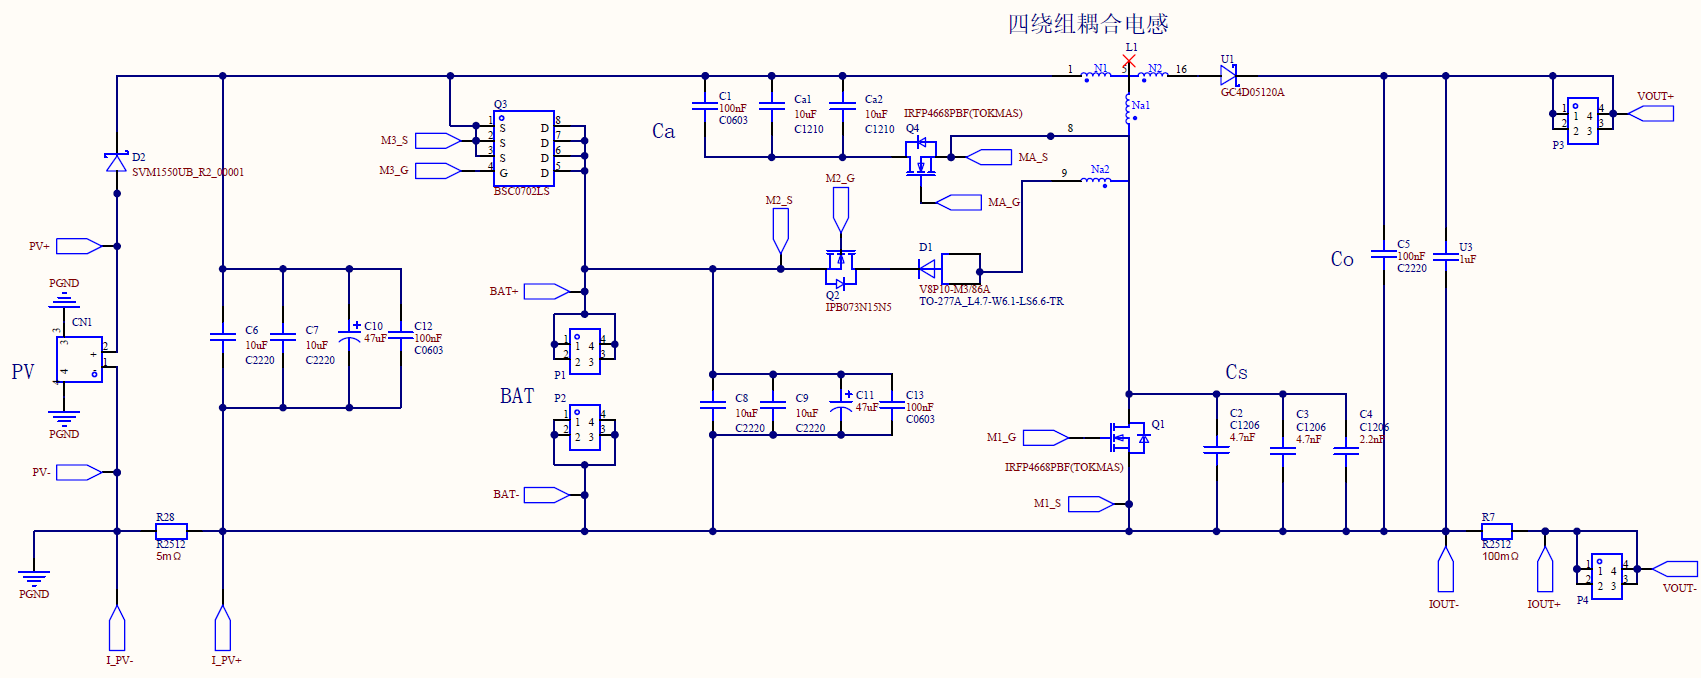
\includegraphics[width=0.95\textwidth]{images/拓扑图/主功率拓扑.png}
  \caption{三端口DC-DC变换器拓扑}
  \label{fig:three_port_topology}
  \vspace{0.2em}
  {\small 资料来源：作者绘制。}
\end{figure}

从主功率器件配置看，功率板中选用了 IRFP4668PBF、IPB073N15N5、BSC0702LS 和 GC4D05120A 等功率器件，用于构成不同端口之间的开关调制通道。功率开关由主控制板输出的 \texttt{PWM\_M1}、\texttt{PWM\_MA}、\texttt{PWM\_M2} 和 \texttt{PWM\_M3} 等信号进行控制。该设计使主控制板能够根据系统运行模式调整不同端口的能量流向，为充电、放电和输出调节等工况提供控制接口。

为满足后续闭环控制和保护判断需求，功率板针对光伏端、输出端和关键器件温度设计了采样接口。采样信号包括光伏输入电压 \texttt{V\_PV}、输出电压 \texttt{V\_OUT}、光伏输入电流 \texttt{I\_PV}、输出电流 \texttt{I\_OUT}、MOSFET 温度 \texttt{TEMP\_MOS} 和磁性器件温度 \texttt{TEMP\_MAG}。其中，电压采样采用高阻分压和运算放大器缓冲方式，将高压侧信号转换至控制器 ADC 可采集范围；电流采样采用分流电阻配合 INA181 电流检测芯片完成信号调理；温度采样用于监测功率器件和磁性器件的热状态。

从原理图可以看出，功率板输出端按照较高电压等级进行设计，因此输出电压采样部分采用多级高阻分压，以降低单个电阻承受的电压应力。采样后端通过 OPA2188 运算放大器进行缓冲和调理，提高采样信号的稳定性和抗干扰能力。电流采样部分通过 \texttt{I\_PV+}、\texttt{I\_PV-}、\texttt{IOUT+} 和 \texttt{IOUT-} 等差分检测节点获取电流信息，再由 INA181 输出与电流成比例的电压信号。该采样链路能够为后续 MPPT、充电限流、放电限流、输出稳压和异常保护提供数据基础。

驱动部分采用 UCC21540ADWKR 隔离驱动芯片，并为各功率开关支路配置隔离电源。隔离驱动能够在控制侧和功率侧之间建立电气隔离，降低高 $dv/dt$ 开关节点对 MCU 控制信号的干扰。驱动网络中设置了栅极电阻、下拉电阻、去耦电容和关断控制信号，用于改善开关速度、抑制误导通并增强故障状态下的关断可靠性。同时，功率板预留了 \texttt{OC\_FAULT} 等故障接口，可与主控制板的 HRTIMER 故障输入配合，在出现过流或异常状态时实现快速关断。

在本阶段，三端口功率变换部分已经完成电路仿真和功率板原理图及 PCB 设计。仿真主要围绕充电、放电和端口切换等典型工况展开，重点观察各端口电压电流变化、功率器件开关状态、耦合电感电流变化以及控制量调节过程。通过仿真可以验证三端口方案在功能逻辑上的可行性，并为后续实物调试提供初始参数参考。

板级实现方面，功率板已经按照主功率回路、采样调理回路和隔离驱动回路进行功能划分。主功率区域围绕四绕组耦合电感和功率开关器件布置，采样区域负责将高压、大电流和温度信号转换为控制器可读取的低压信号，驱动区域负责接收主控制板 PWM 信号并驱动功率器件。该划分有利于降低控制信号与功率开关噪声之间的相互干扰，也便于后续分模块调试。

需要说明的是，当前三端口功率板已经完成仿真和板级设计，但实物测试仍需进一步开展。后续测试将按照由低压到高压、由开环到闭环、由单端口到多端口协同的顺序推进。首先验证隔离驱动、电源、采样和保护接口是否正常；随后在限压限流条件下测试单端口能量传递和开关波形；最后逐步开展充放电闭环、输出稳压和多模式切换测试。通过这种分阶段测试方式，可以降低功率级调试风险，并逐步验证三端口方案在实际硬件中的可行性。

综上，三端口功率变换平台已完成硬件设计与基础功能验证（PV$\rightarrow$Battery 充电功能），但 PV$\rightarrow$Load、Battery$\rightarrow$Load 及多模式能量流控制等完整功能仍需后续阶段进一步验证。该平台为后续闭环控制和整机能量调度提供了统一硬件基础。

\subsection{本章小结}

本章对系统总体方案与芯片分工进行了论证。三节点协同架构实现了控制、保护、转发和监控的解耦，三端口功率变换平台已完成硬件设计与基础功能验证。后续章节将进一步展开硬件设计、软件流程与测试验证。
